\apendice{Especificación de Requisitos}

Si procede.

\section{Descripción requisitos funcionales}

\begin{itemize}
    \item \textbf{RF-01 Iniciar sesión}: Todos los usuarios deben introducir de forma obligatoria su correo electrónico, tipo de usuario y contraseña para poder acceder a la página web.
    \item \textbf{RF-02 Consultar pacientes y usuarios}: Otorgar acceso a la lista completa de usuarios o pacientes, según los permisos asignados al usuario, y permitir la realización de búsquedas específicas dentro de ella.
    \item \textbf{RF-03 Gestionar pacientes y usuarios}: Permitir la creación y eliminación de cuentas, así como la modificación de los datos almacenados en las cuentas de pacientes y médicos. La capacidad para realizar estas acciones depende del nivel de acceso que el usuario tenga en el sistema web.
    \item \textbf{RF-04 Realizar actividad}: Ofrece las opciones de iniciar y finalizar actividades, así como la opción de guardar o descartar estas mismas. Existirá la posibilidad de realización de actividades sin que exista conexión entre el dispositivo físico y la página web, el denominado "modo offline".
    \item \textbf{RF-05 Mostrar actividades}: Presenta al usuario las actividades realizadas por el paciente, ya sea a través de un calendario de actividades o una lista con aquellas que cumplen unos criterios establecidos por el propio usuario.
    \item \textbf{RF-06 Consultar estadísticas}: Visualización de los datos relacionados con las actividades realizadas por el paciente, ya sea de una actividad en concreto o de todas en conjunto.
    \item \textbf{RF-07 Gestionar cuenta}: Facilitar a los usuarios las tareas de cambio de contraseña y actualización del correo eléctrónico vinculado a su cuenta.
    \item \textbf{RF-08 Cerrar sesión}: Todos los usuarios tendrán la opción de cerrar sesión desde el menú de inicio. Para prevenir cierres accidentales, se solicitará una confirmación de la acción antes de que esta se complete.
\end{itemize}


\section{Diagrama de casos de uso}


\begin{figure}[h]
    \centering
    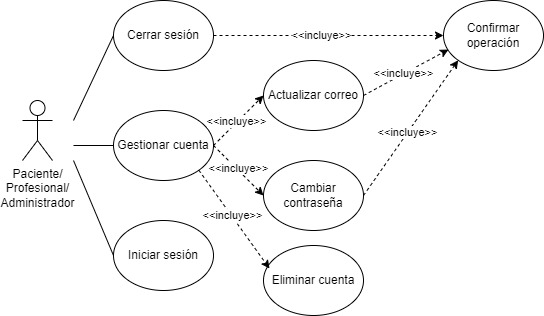
\includegraphics[width=1\textwidth]{img/CUdiagramas/CU-todos.jpg}
    \caption{CU-todos}
    \label{fig:CU-todos}
\end{figure}

\begin{figure}[h]
    \centering
    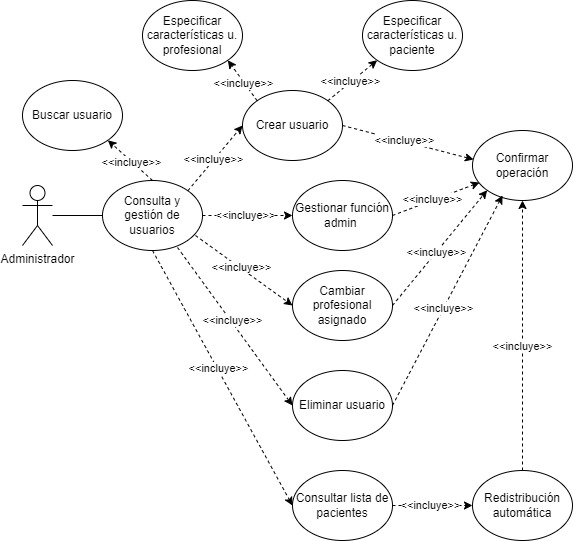
\includegraphics[width=1\textwidth]{img/CUdiagramas/CU-Administrador.jpg}
    \caption{CU-Administrador}
    \label{fig:CU-Administrador}
\end{figure}

\begin{figure}[h]
    \centering
    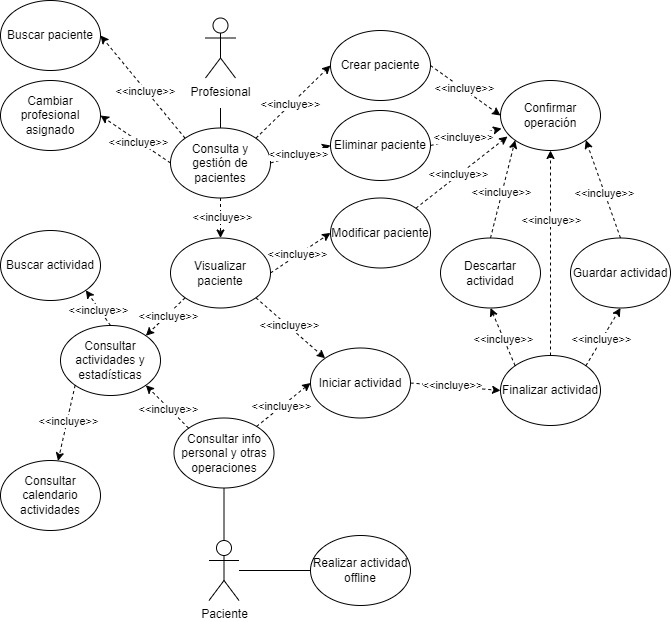
\includegraphics[width=1\textwidth]{img/CUdiagramas/CU-Paciente_Profesional.jpg}
    \caption{CU-Pacientes y Profesionales}
    \label{fig:CU-Paciente_Profesional}
\end{figure}




\section{Explicación casos de uso.}

Se puede describir mediante el uso de tablas o mediante lenguaje natural.    

Una muestra de cómo podría ser una tabla de casos de uso:

% Caso de Uso 1 -> Iniciar sesión. -> ACABADO
\begin{table}[p]
	\centering
	\begin{tabularx}{\linewidth}{ p{0.21\columnwidth} p{0.71\columnwidth} }
		\toprule
		\textbf{CU-1}    & \textbf{Iniciar sesión}\\
		\toprule
        \textbf{Versión}              & 1.0    \\
		\textbf{Autor}                & Inés Martos Barbero \\
		\textbf{Requisitos asociados} & RF-01 \\
		\textbf{Descripción}          & Acceso del usuario al sistema mediante la selección del tipo de usuario y la autenticación de correo electrónico y contraseña. \\
		\textbf{Precondición}         & El usuario debe estar dado de alta en el sistema. \\
		\textbf{Acciones}             &
		\begin{enumerate}
			\def\labelenumi{\arabic{enumi}.}
			\tightlist
			\item Seleccionar tipo de usuario: paciente/profesional/administrador
			\item Ingresar credenciales (correo electrónico y contraseña)
            \item Validar credenciales
		\end{enumerate}\\
		\textbf{Postcondiciones}        & 
        \begin{enumerate}
			\def\labelenumi{\arabic{enumi}.}
			\tightlist
			\item Acceso al sistema concedido
			\item Inicio de sesión registrado para propósitos de seguimiento y seguridad
		\end{enumerate}\\
		\textbf{Excepciones}          & 
        \begin{enumerate}
			\def\labelenumi{\arabic{enumi}.}
			\tightlist
            \item Tipo de usuario no seleccionado. Alerta indicando que es necesaria la selección
            \item Ausencia de credenciales. El sistema pide que se completen los campos de correo electrónico y contraseña
			\item Credenciales incorrectas. Mensaje de aviso y permitir hasta 3 nuevos intentos
			\item Múltiples intentos fallidos. La cuenta será bloqueada un total de 5 minutos por seguridad
		\end{enumerate}\\
		\textbf{Importancia}          & Alta \\
		\bottomrule
	\end{tabularx}
	\caption{CU-1 Iniciar sesión.}
\end{table}

% Caso de Uso 2 -> Confirmar operación. -> ACABADO
\begin{table}[p]
	\centering
	\begin{tabularx}{\linewidth}{ p{0.21\columnwidth} p{0.71\columnwidth} }
		\toprule
		\textbf{CU-2}    & \textbf{Confirmar operación}\\
		\toprule
        \textbf{Versión}              & 1.0    \\
		\textbf{Autor}                & Inés Martos Barbero \\
		\textbf{Requisitos asociados} & RF-03, RF-04, RF-07, RF-08 \\
		\textbf{Descripción}          & Verificación y aprobación de acciones críticas o cambios significativos en el sistema. \\
		\textbf{Precondición}         & Operación pendiente de confirmación \\
		\textbf{Acciones}             &
		\begin{enumerate}
			\def\labelenumi{\arabic{enumi}.}
			\tightlist
			\item El sistema muestra al usuario una ventana emergente para que este confirme la operación
			\item Confirmación o rechazo de la operación a través de un clic
		\end{enumerate}\\
		\textbf{Postcondición}        & Operación confirmada y llevada a cabo \\
        \textbf{Excepción}            & Operación cancelada. El sistema devuelve al usuario a la pantalla anterior sin realizar el cambio que se iba a llevar a cabo \\
		\textbf{Importancia}          & Media \\
		\bottomrule
	\end{tabularx}
	\caption{CU-2 Confirmar operación.}
\end{table}

% Caso de Uso 3 -> Gestionar cuenta. -> ACABADO
\begin{table}[p]
	\centering
	\begin{tabularx}{\linewidth}{ p{0.21\columnwidth} p{0.71\columnwidth} }
		\toprule
		\textbf{CU-3}    & \textbf{Gestionar cuenta}\\
		\toprule
		\textbf{Versión}              & 1.0    \\
		\textbf{Autor}                & Inés Martos Barbero \\
		\textbf{Requisitos asociados} & RF-07 \\
		\textbf{Descripción}          & Administración de las credenciales del usuario necesarias para el inicio de sesión \\
		\textbf{Precondición}         & Usuario autenticado \\
		\textbf{Acciones}             &
		\begin{enumerate}
			\def\labelenumi{\arabic{enumi}.}
			\tightlist
			\item Acceso a la ventana de gestión de la cuenta y presentación de las opciones que esta ofrece
			\item Selección de la operación que se quiere realizar; CU-4 Actualizar correo, CU-5 Cambiar contraseña
		\end{enumerate}\\ 
		\textbf{Postcondiciones}        &
		\begin{enumerate}
			\def\labelenumi{\arabic{enumi}.}
			\tightlist
			\item Visualización de la información de la cuenta y las opciones disponibles.
			\item Redirección a casos de uso específicos
		\end{enumerate}\\
		\textbf{Excepción}          & El usuario puede decidir no realizar ninguna de las operaciones y regresar a la pantalla anterior, página de inicio o cualquiera de las opciones del menú principal \\
		\textbf{Importancia}          & Media \\
		\bottomrule
	\end{tabularx}
	\caption{CU-3 Gestionar cuenta.}
\end{table}


% Caso de Uso 4 -> Actualizar correo. -> ACABADO
\begin{table}[p]
	\centering
	\begin{tabularx}{\linewidth}{ p{0.21\columnwidth} p{0.71\columnwidth} }
		\toprule
		\textbf{CU-4}    & \textbf{Actualizar correo}\\
		\toprule
		\textbf{Versión}              & 1.0    \\
		\textbf{Autor}                & Inés Martos Barbero \\
		\textbf{Requisitos asociados} & RF-07 \\
		\textbf{Descripción}          & Cambio del correo electrónico asociado a la cuenta del usuario \\
		\textbf{Precondición}         & Redirección desde 'Gestionar Cuenta' CU-3 \\
		\textbf{Acciones}             &
		\begin{enumerate}
			\def\labelenumi{\arabic{enumi}.}
			\tightlist
			\item Introducir la nueva dirección de correo en el campo correspondiente
			\item Verificación del nuevo correo introducido. El sistema solicita al usuario que reingrese el correo para confirmar que es el correcto.
                \item Seleccionar de la opción 'aplicar cambios'
                \item Confirmación de la operación, CU-2
		\end{enumerate}\\
		\textbf{Postcondiciones}        &
		\begin{enumerate}
			\def\labelenumi{\arabic{enumi}.}
			\tightlist
			\item Actualización del correo electrónico y notificación de operación exitosa
                \item Redirección a la ventana de Gestión de la cuenta (CU-2, CU-3)
		\end{enumerate}\\
		\textbf{Excepciones}          & 
            \begin{enumerate}
			\def\labelenumi{\arabic{enumi}.}
			\tightlist
			\item Campo vacío. Solicitar al usuario que introduzca la dirección de correo en los dos campos habilitados para ello
                \item Error de verificación: los correos introducidos no coinciden. Situación comunicada al usuario para que este actúe en consecuencia
                \item Formato de correo electrónico no válido. El sistema informa al usuario, solicita modificación y no se permite el cambio
                \item Correo electrónico en uso. La dirección de correo introducida ya se encuentra asociada a otra cuenta. Se informa del problema al usuario y no se permite el cambio
                \item Botón 'Cancelar operación' redirecciona a la pantalla de 'Gestión de la cuenta'
		\end{enumerate}\\
		\textbf{Importancia}          & Baja \\
		\bottomrule
	\end{tabularx}
	\caption{CU-4 Actualizar correo.}
\end{table}

% Caso de Uso 5 -> Cambiar contraseña. -> ACABADO
\begin{table}[p]
	\centering
	\begin{tabularx}{\linewidth}{ p{0.21\columnwidth} p{0.71\columnwidth} }
		\toprule
		\textbf{CU-5}    & \textbf{Cambiar contraseña}\\
		\toprule
		\textbf{Versión}              & 1.0    \\
		\textbf{Autor}                & Inés Martos Barbero \\
		\textbf{Requisitos asociados} & RF-07 \\
		\textbf{Descripción}          & Modificación de la contraseña actual del usuario \\
		\textbf{Precondición}         & Redirección desde 'Gestionar Cuenta' CU-3 \\
		\textbf{Acciones}             &
		\begin{enumerate}
			\def\labelenumi{\arabic{enumi}.}
			\tightlist
			\item Ingresar la contraseña actual para verificar la identidad del usuario
                \item Introducir nueva contraseña en el campo correspondiente
                \item Repetir contraseña
			\item Seleccionar de la opción 'aplicar cambios'
                \item Confirmación de la operación, CU-2
		\end{enumerate}\\
		\textbf{Postcondiciones}        &
		\begin{enumerate}
			\def\labelenumi{\arabic{enumi}.}
			\tightlist
			\item Actualización de la contraseña y notificación de operación exitosa
                \item Redirección a la ventana de Gestión de la cuenta (CU-2, CU-3)
		\end{enumerate}\\
		\textbf{Excepciones}          & 
            \begin{enumerate}
			\def\labelenumi{\arabic{enumi}.}
			\tightlist
			\item Campo vacío. Solicitar al usuario que rellene todos los campos
                \item Contraseña actual incorrecta. Notificación al usuario y solicitud para que se vuelva a introducir
                \item Error de verificación. Las nuevas contraseñas introducidas no coinciden entre sí. Se informa al usuario y se solicita modificación
                \item Botón 'Cancelar operación' redirecciona a la pantalla de 'Gestión de la cuenta'
		\end{enumerate}\\
		\textbf{Importancia}          & Baja \\
		\bottomrule
	\end{tabularx}
	\caption{CU-5 Cambiar contraseña.}
\end{table}

% Caso de Uso 6 -> Cerrar sesión. -> ACABADO
\begin{table}[p]
	\centering
	\begin{tabularx}{\linewidth}{ p{0.21\columnwidth} p{0.71\columnwidth} }
		\toprule
		\textbf{CU-6}    & \textbf{Cerrar sesión}\\
		\toprule
		\textbf{Versión}              & 1.0    \\
		\textbf{Autor}                & Inés Martos Barbero \\
		\textbf{Requisitos asociados} & RF-08 \\
		\textbf{Descripción}          & Desconexión segura del usuario del sistema \\
		\textbf{Precondición}         & Usuario autenticado (sesión iniciada) \\
		\textbf{Acciones}             &
		\begin{enumerate}
			\def\labelenumi{\arabic{enumi}.}
			\tightlist
			\item Selección de 'Cerrar Sesión' desde la opción del menú principal
			\item Confirmar operación, CU-2
		\end{enumerate}\\
		\textbf{Postcondiciones}        & 
            \begin{enumerate}
			\def\labelenumi{\arabic{enumi}.}
			\tightlist
			\item Sesión Cerrada
			\item Redirección a la pantalla de inicio de sesión (CU-1)
		\end{enumerate}\\
		\textbf{Excepción}          & Operación cancelada desde CU-2  \\
		\textbf{Importancia}          & Alta  \\
		\bottomrule
	\end{tabularx}
	\caption{CU-6 Cerrar sesión.}
\end{table}

% Caso de Uso 7 -> Consulta y gestión de usuarios.
\begin{table}[p]
	\centering
	\begin{tabularx}{\linewidth}{ p{0.21\columnwidth} p{0.71\columnwidth} }
		\toprule
		\textbf{CU-7}    & \textbf{Consulta y gestión de usuarios}\\
		\toprule
		\textbf{Versión}              & 1.0    \\
		\textbf{Autor}                & Inés Martos Barbero \\
		\textbf{Requisitos asociados} & RF-02, RF-03 \\
		\textbf{Descripción}          & Revisión y manejo de los datos de los usuarios registrados en el sistema \\
		\textbf{Precondición}         & Precondiciones (podría haber más de una) \\
		\textbf{Acciones}             &
		\begin{enumerate}
			\def\labelenumi{\arabic{enumi}.}
			\tightlist
			\item Pasos del CU
			\item Pasos del CU (añadir tantos como sean necesarios)
		\end{enumerate}\\
		\textbf{Postcondición}        & Postcondiciones (podría haber más de una) \\
		\textbf{Excepciones}          & Excepciones \\
		\textbf{Importancia}          & Alta o Media o Baja... \\
		\bottomrule
	\end{tabularx}
	\caption{CU-7 Consulta y gestión de usuarios.}
\end{table}

% Caso de Uso 8 -> Buscar usuario.  -> ACABADO
\begin{table}[p]
	\centering
	\begin{tabularx}{\linewidth}{ p{0.21\columnwidth} p{0.71\columnwidth} }
		\toprule
		\textbf{CU-8}    & \textbf{Buscar usuario}\\
		\toprule
		\textbf{Versión}              & 1.0    \\
		\textbf{Autor}                & Inés Martos Barbero \\
		\textbf{Requisitos asociados} & RF-02 \\
		\textbf{Descripción}          & Localización de usuarios dentro del sistema a través de nombre, apellidos, email y tipo de usuario \\
		\textbf{Precondiciones}         & 
            \begin{enumerate}
			\def\labelenumi{\arabic{enumi}.}
			\tightlist
			\item Usuario de tipo administrador autenticado
			\item Acceso desde la pantalla de inicio
		\end{enumerate}\\
		\textbf{Acciones}             &
		\begin{enumerate}
			\def\labelenumi{\arabic{enumi}.}
			\tightlist
			\item Ingreso de los criterios de búsqueda. Se pueden introducir escribiéndolos (nombre, apellidos o correo electrónico) o por selección del tipo de usuario a través de un desplegable
			\item Envío de la solicitud de búsqueda. Botón lupa o 'buscar' para la obtención de los resultados
		\end{enumerate}\\
		\textbf{Postcondiciones}        & 
            \begin{enumerate}
			\def\labelenumi{\arabic{enumi}.}
			\tightlist
			\item Presentación de una lista de usuarios que cumplen con los criterios de búsqueda. Se muestra su nombre, apellidos, correo y rol.
			\item Gestión de usuarios encontrados: eliminar y modificar. Seguirá apareciendo la opción de crear usuario
                \item Opción de eliminar el filtro aplicado y volver a mostrar todos los usuarios. Botón 'Eliminar filtro'
		\end{enumerate}\\
		\textbf{Excepciones}          & 
            \begin{enumerate}
			\def\labelenumi{\arabic{enumi}.}
			\tightlist
			\item 
			\item Búsqueda sin resultados
                \item Error por formato erróneo del correo electrónico introducido
		\end{enumerate}\\
		\textbf{Importancia}          & Media \\
		\bottomrule
	\end{tabularx}
	\caption{CU-8 Buscar usuario.}
\end{table}

\section{Prototipos de interfaz o interacción con el proyecto.}

\subsection{Wireframes}

% Iniciar sesión
\begin{figure}[h]
    \centering
    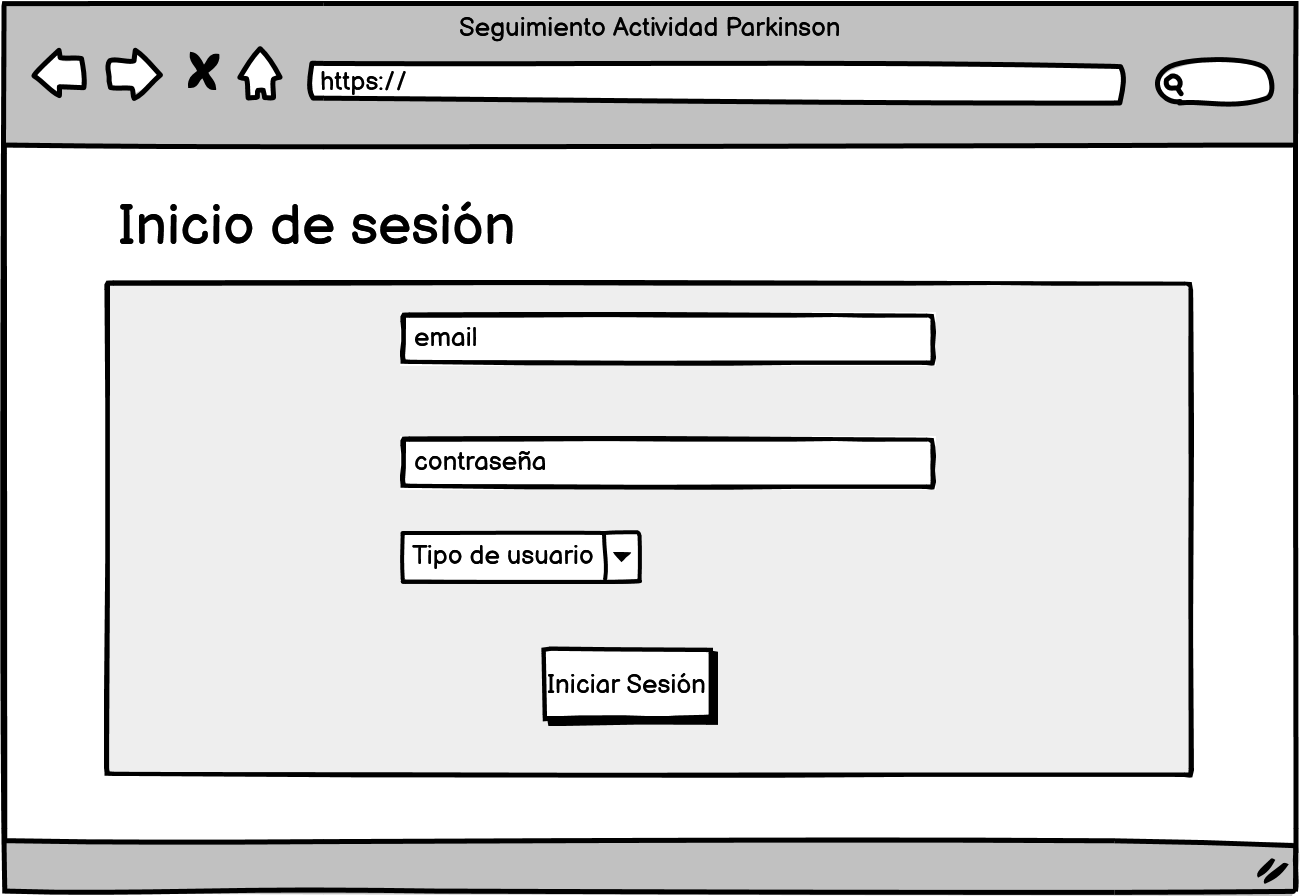
\includegraphics[width=1\textwidth]{img/UI_Wireframes/UI_CU-1_Iniciar sesión.png}
    \caption{Iniciar sesión}
    \label{fig:Iniciar sesión}
\end{figure}

% Confirmar operación
\begin{figure}[h]
    \centering
    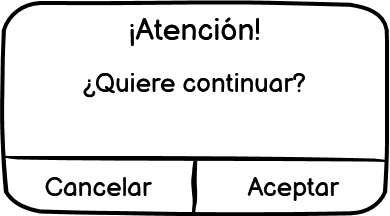
\includegraphics[width=0.4\textwidth]{img/UI_Wireframes/UI_CU-2_Confirmar operación.png}
    \caption{Confirmar operación}
    \label{fig:Confirmar operación}
\end{figure}

% Consulta y gestión de usuarios
\begin{figure}[h]
    \centering
    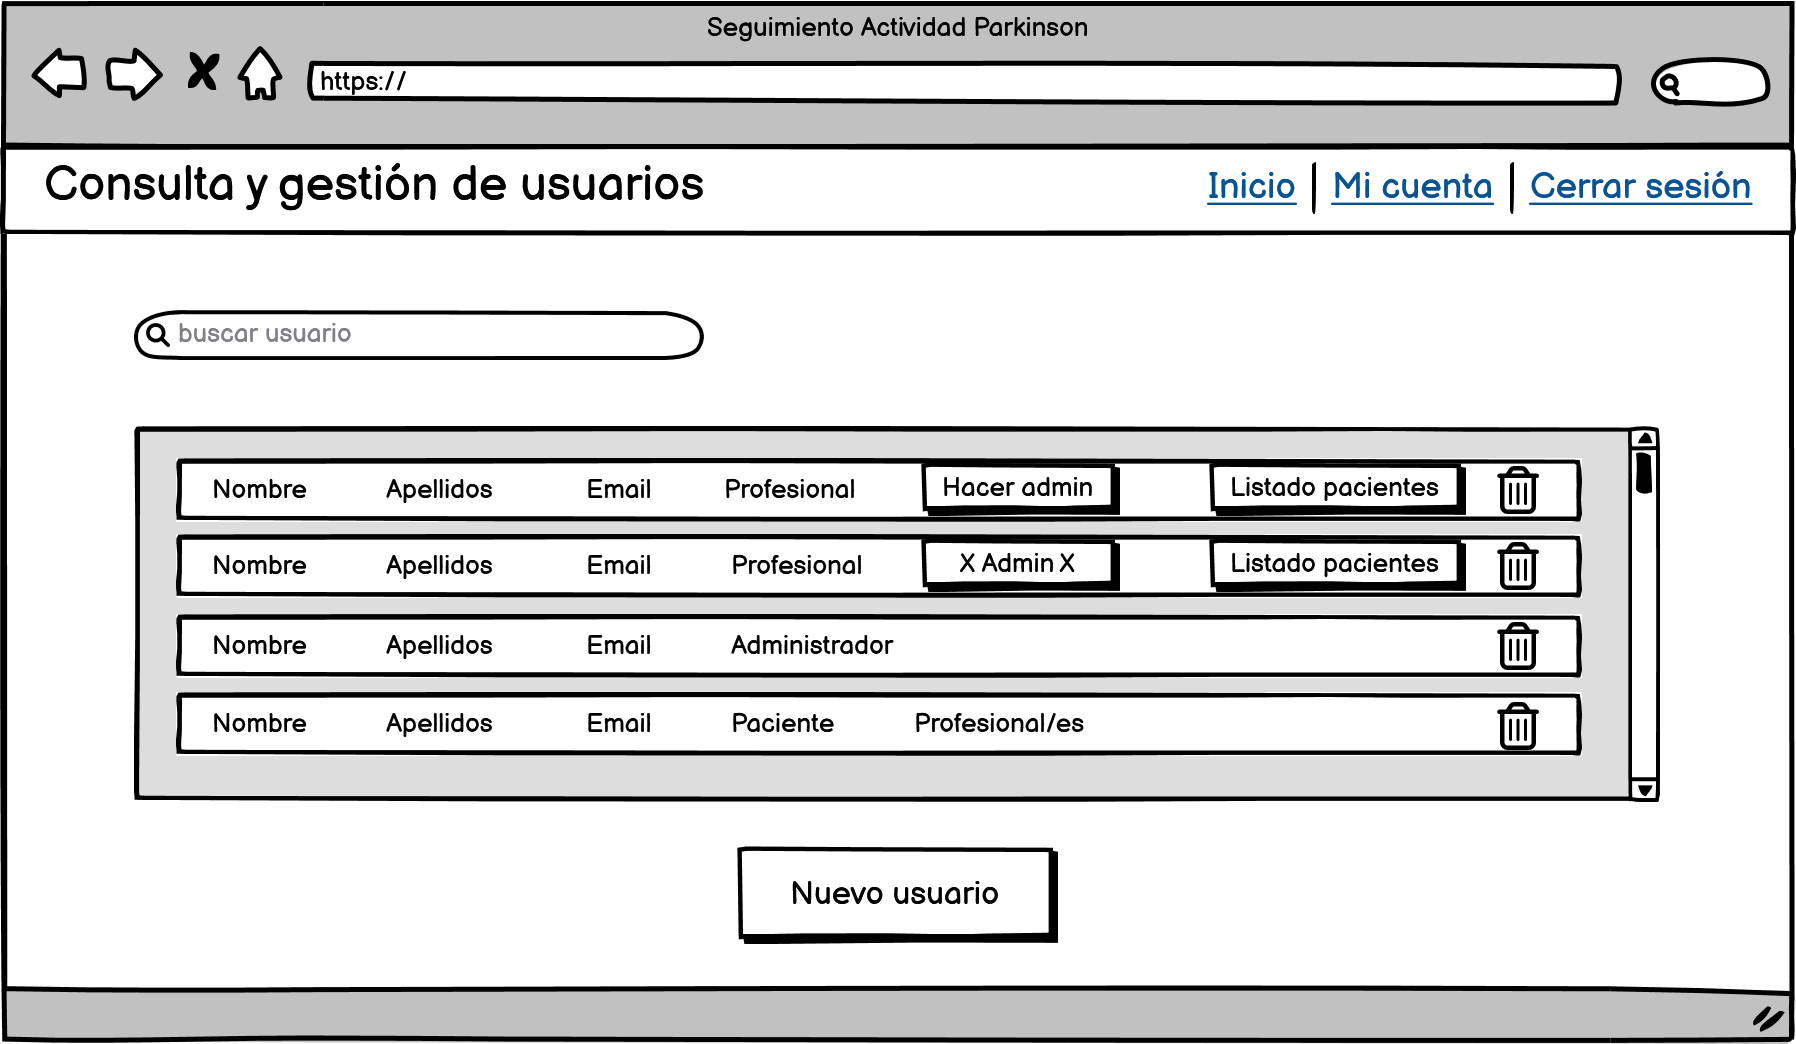
\includegraphics[width=1\textwidth]{img/UI_Wireframes/UI_CU-7_Consulta y gestión de usuarios.png}
    \caption{Consulta y gestión de usuarios}
    \label{fig:Consulta y gestión de usuarios}
\end{figure}

% Crear usuario
\begin{figure}[h]
    \centering
    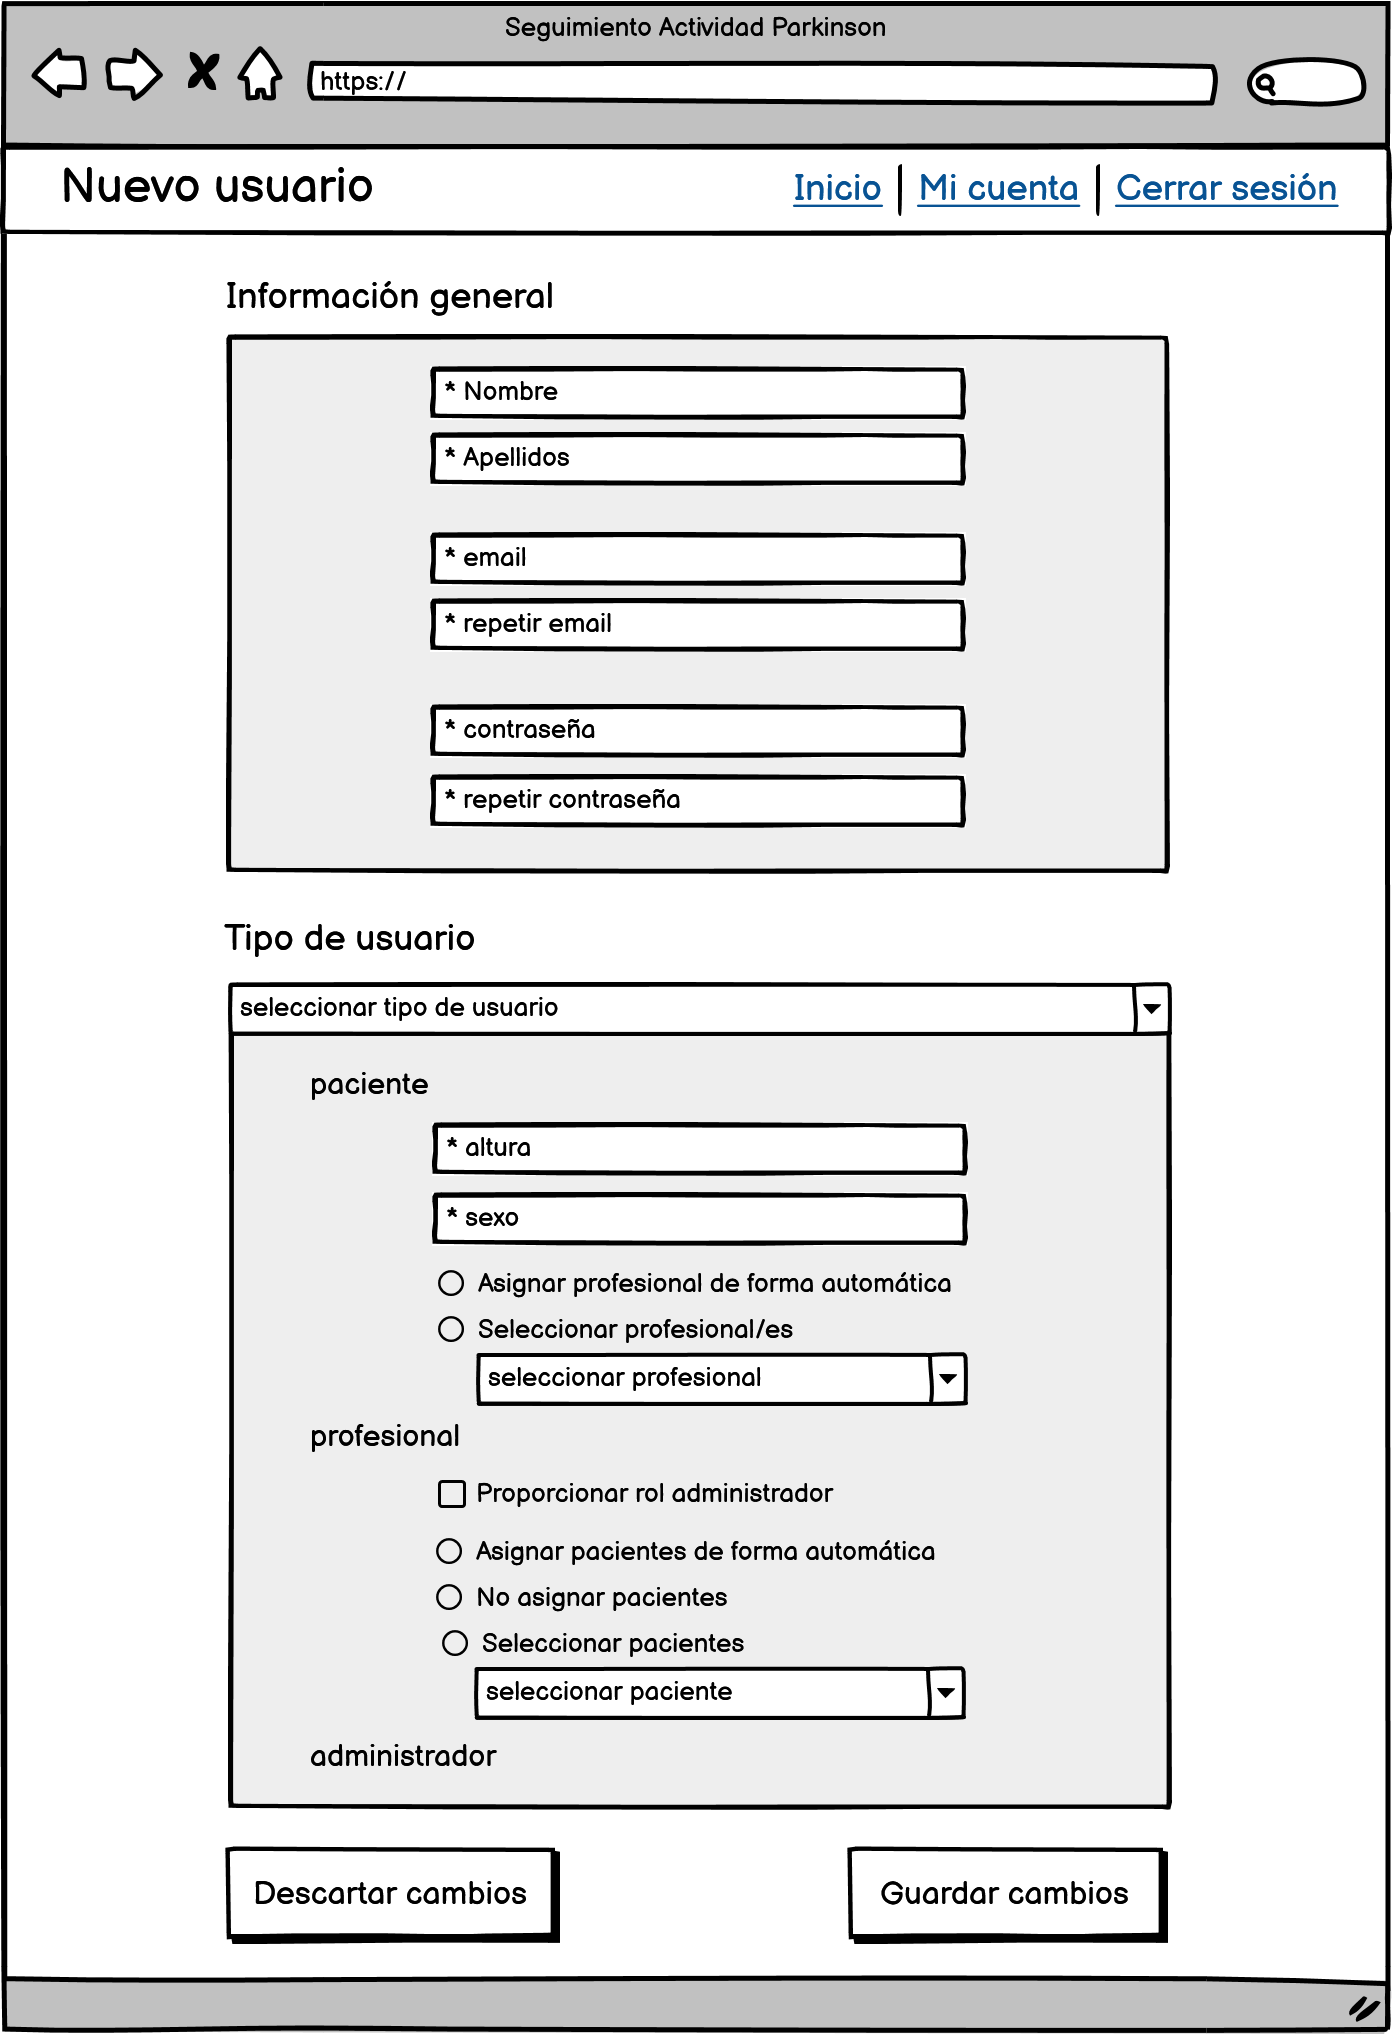
\includegraphics[width=1\textwidth]{img/UI_Wireframes/UI_CU-9_Crear usuario.png}
    \caption{Crear usuario}
    \label{fig:Crear usuario}
\end{figure}

% Consultar lista de pacientes
\begin{figure}[h]
    \centering
    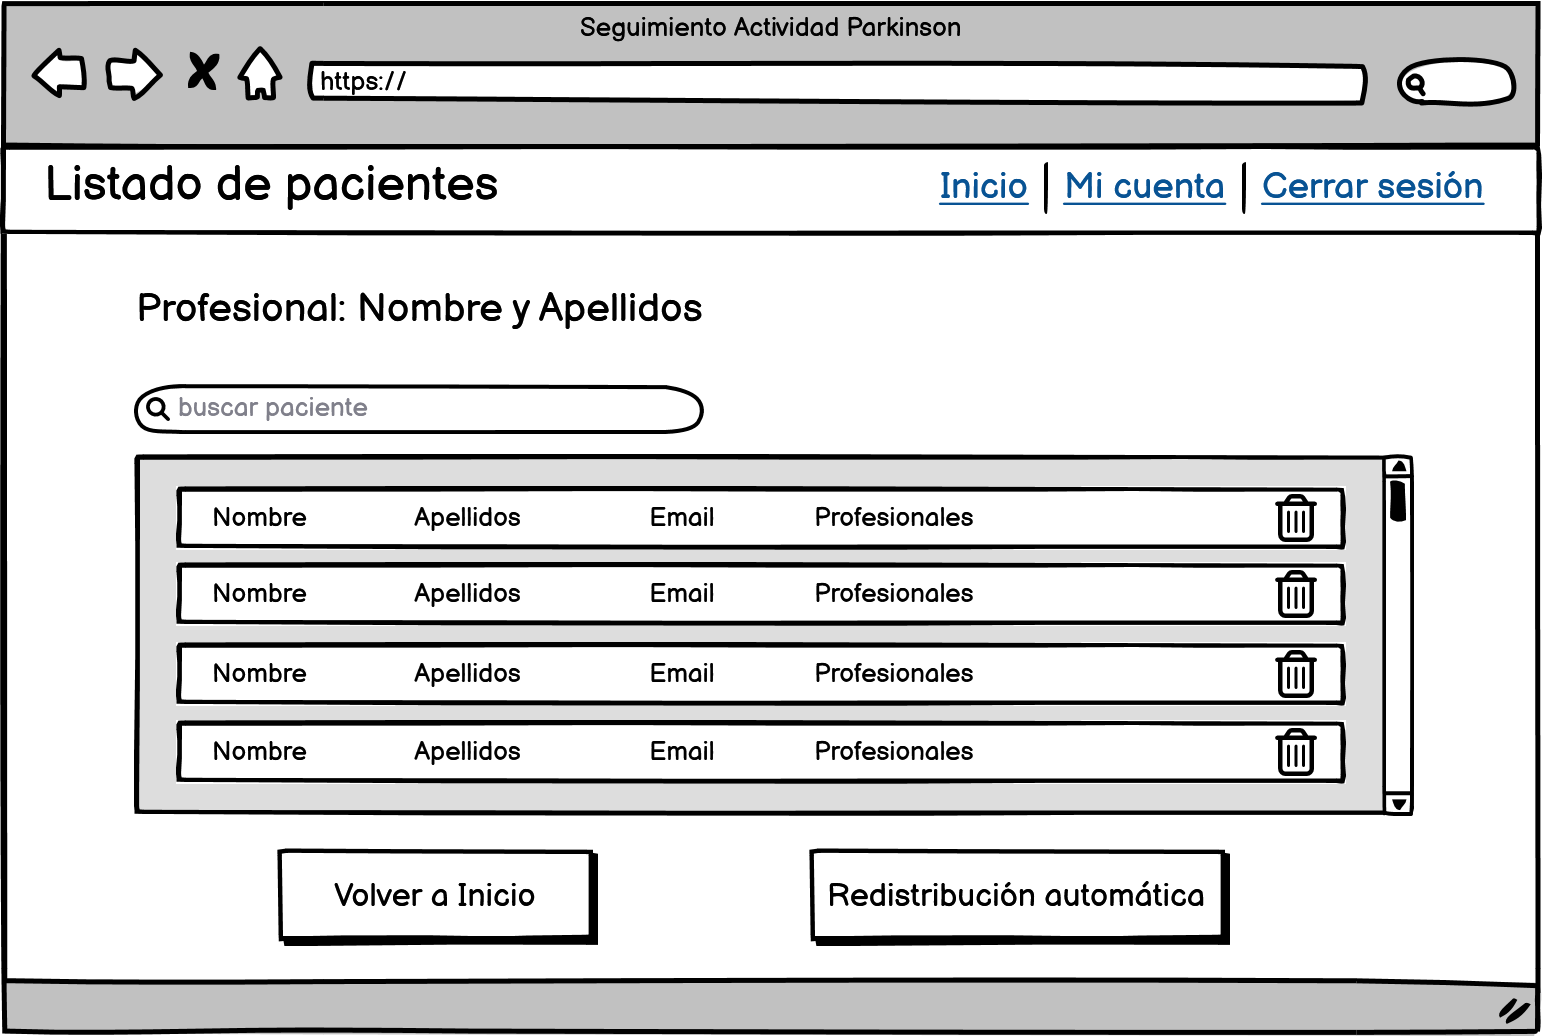
\includegraphics[width=1\textwidth]{img/UI_Wireframes/UI_CU-15_Consultar lista de pacientes.png}
    \caption{Consultar lista de pacientes}
    \label{fig:Consultar lista de pacientes}
\end{figure}

% Consultar información personal y otras operaciones
\begin{figure}[h]
    \centering
    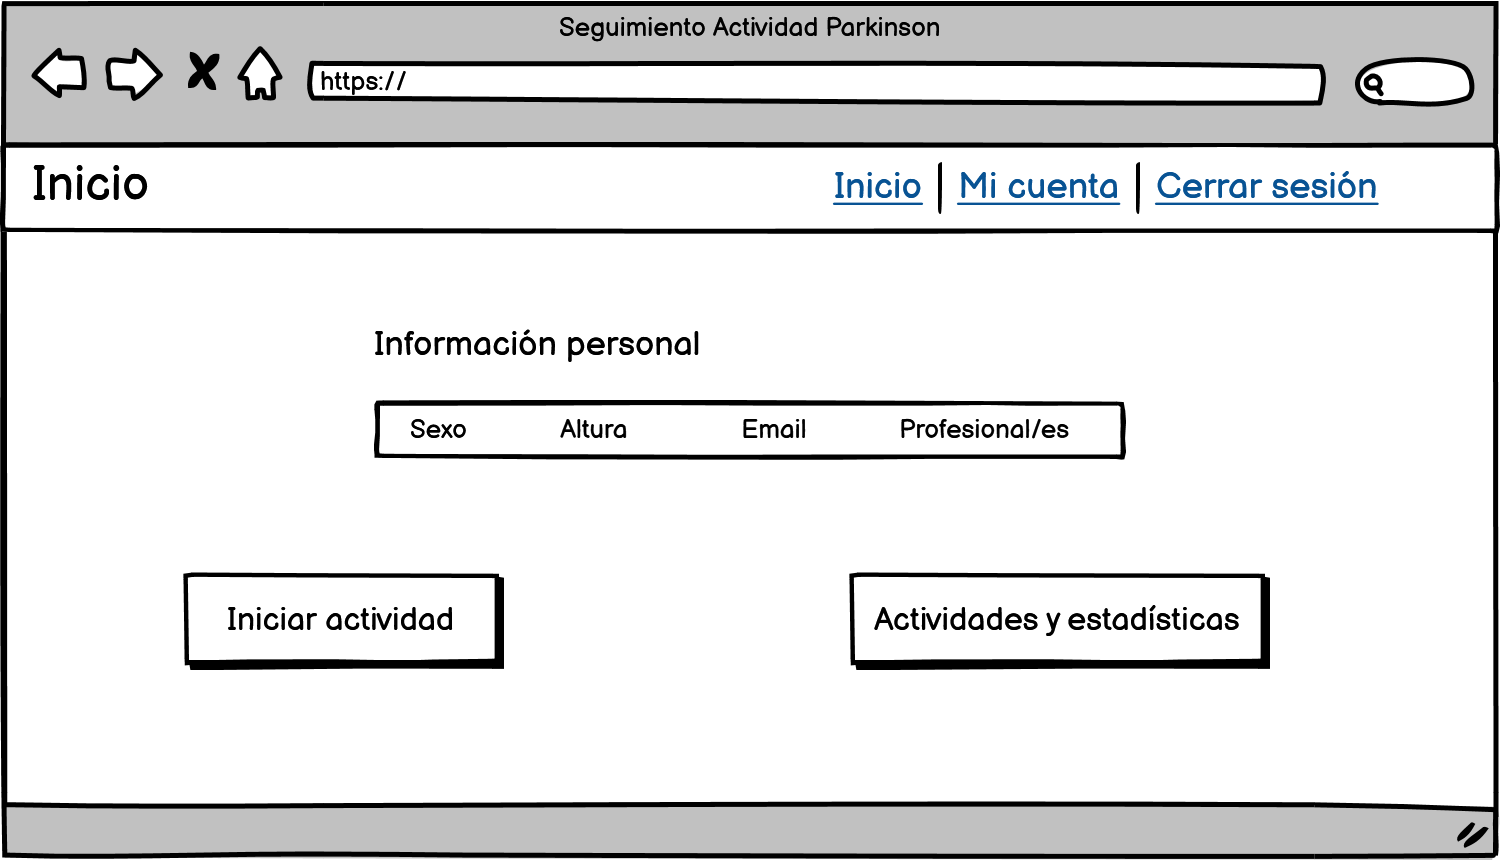
\includegraphics[width=1\textwidth]{img/UI_Wireframes/UI_CU-17_Consultar info personal y otras actividades.png}
    \caption{Consultar información personal y otras actividades}
    \label{fig:Consultar info personal y otras actividades}
\end{figure}

% Iniciar actividad
\begin{figure}[h]
    \centering
    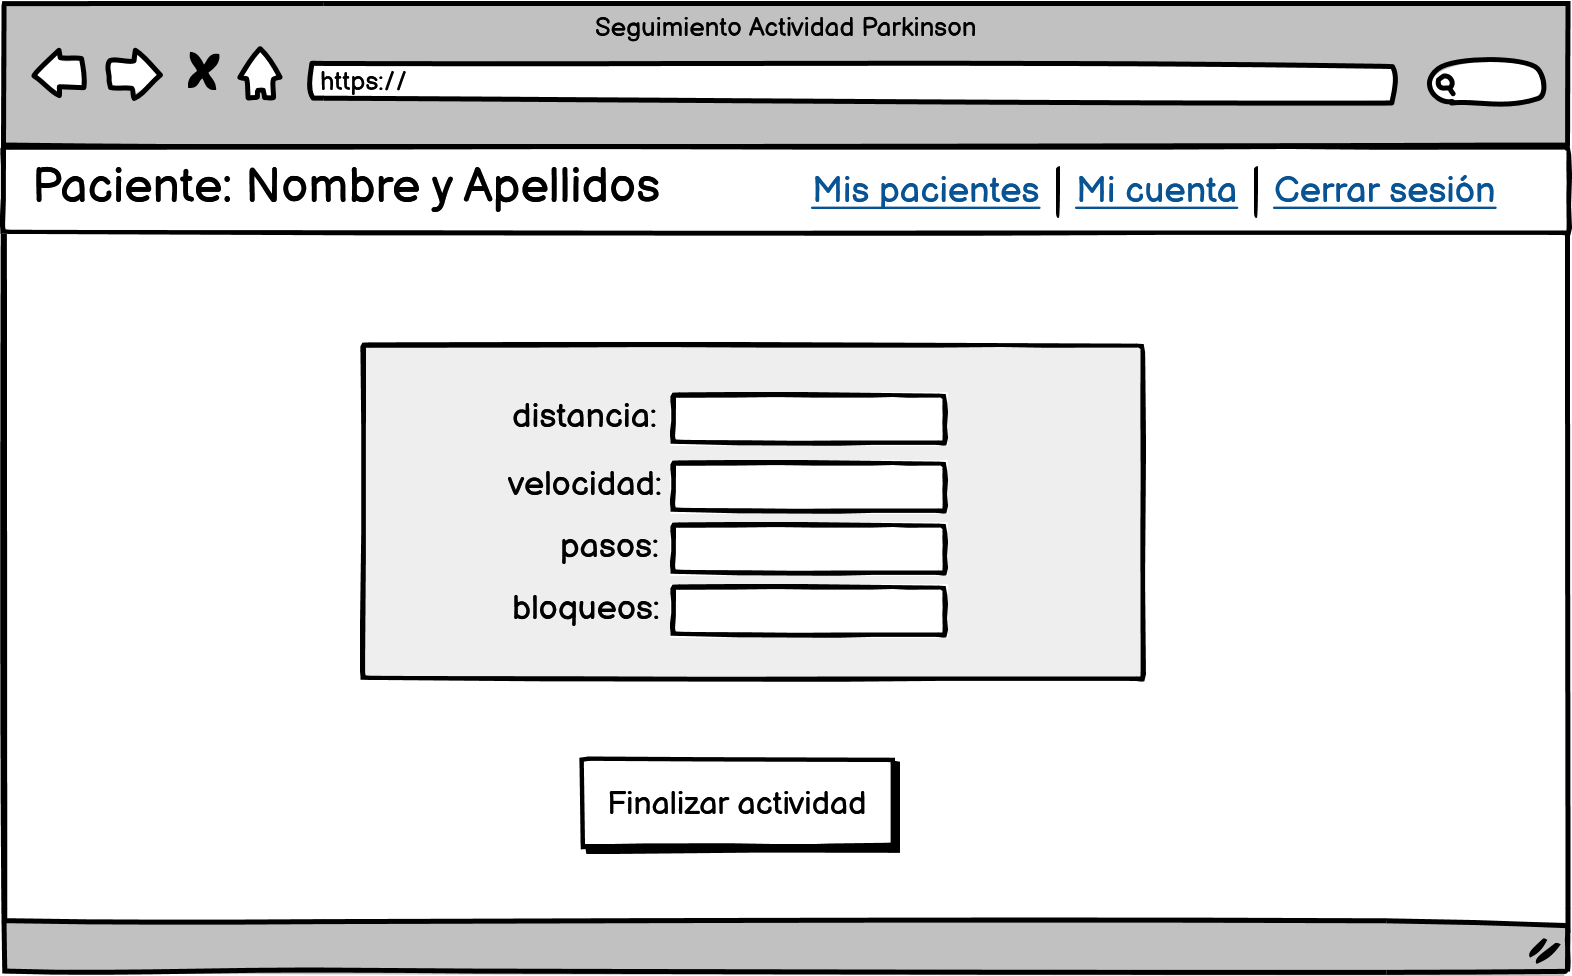
\includegraphics[width=1\textwidth]{img/UI_Wireframes/UI_CU-19_Iniciar actividad.png}
    \caption{Iniciar actividad}
    \label{fig:Iniciar actividad}
\end{figure}

% Consultar actividades y estadísticas (Paciente)
\begin{figure}[h]
    \centering
    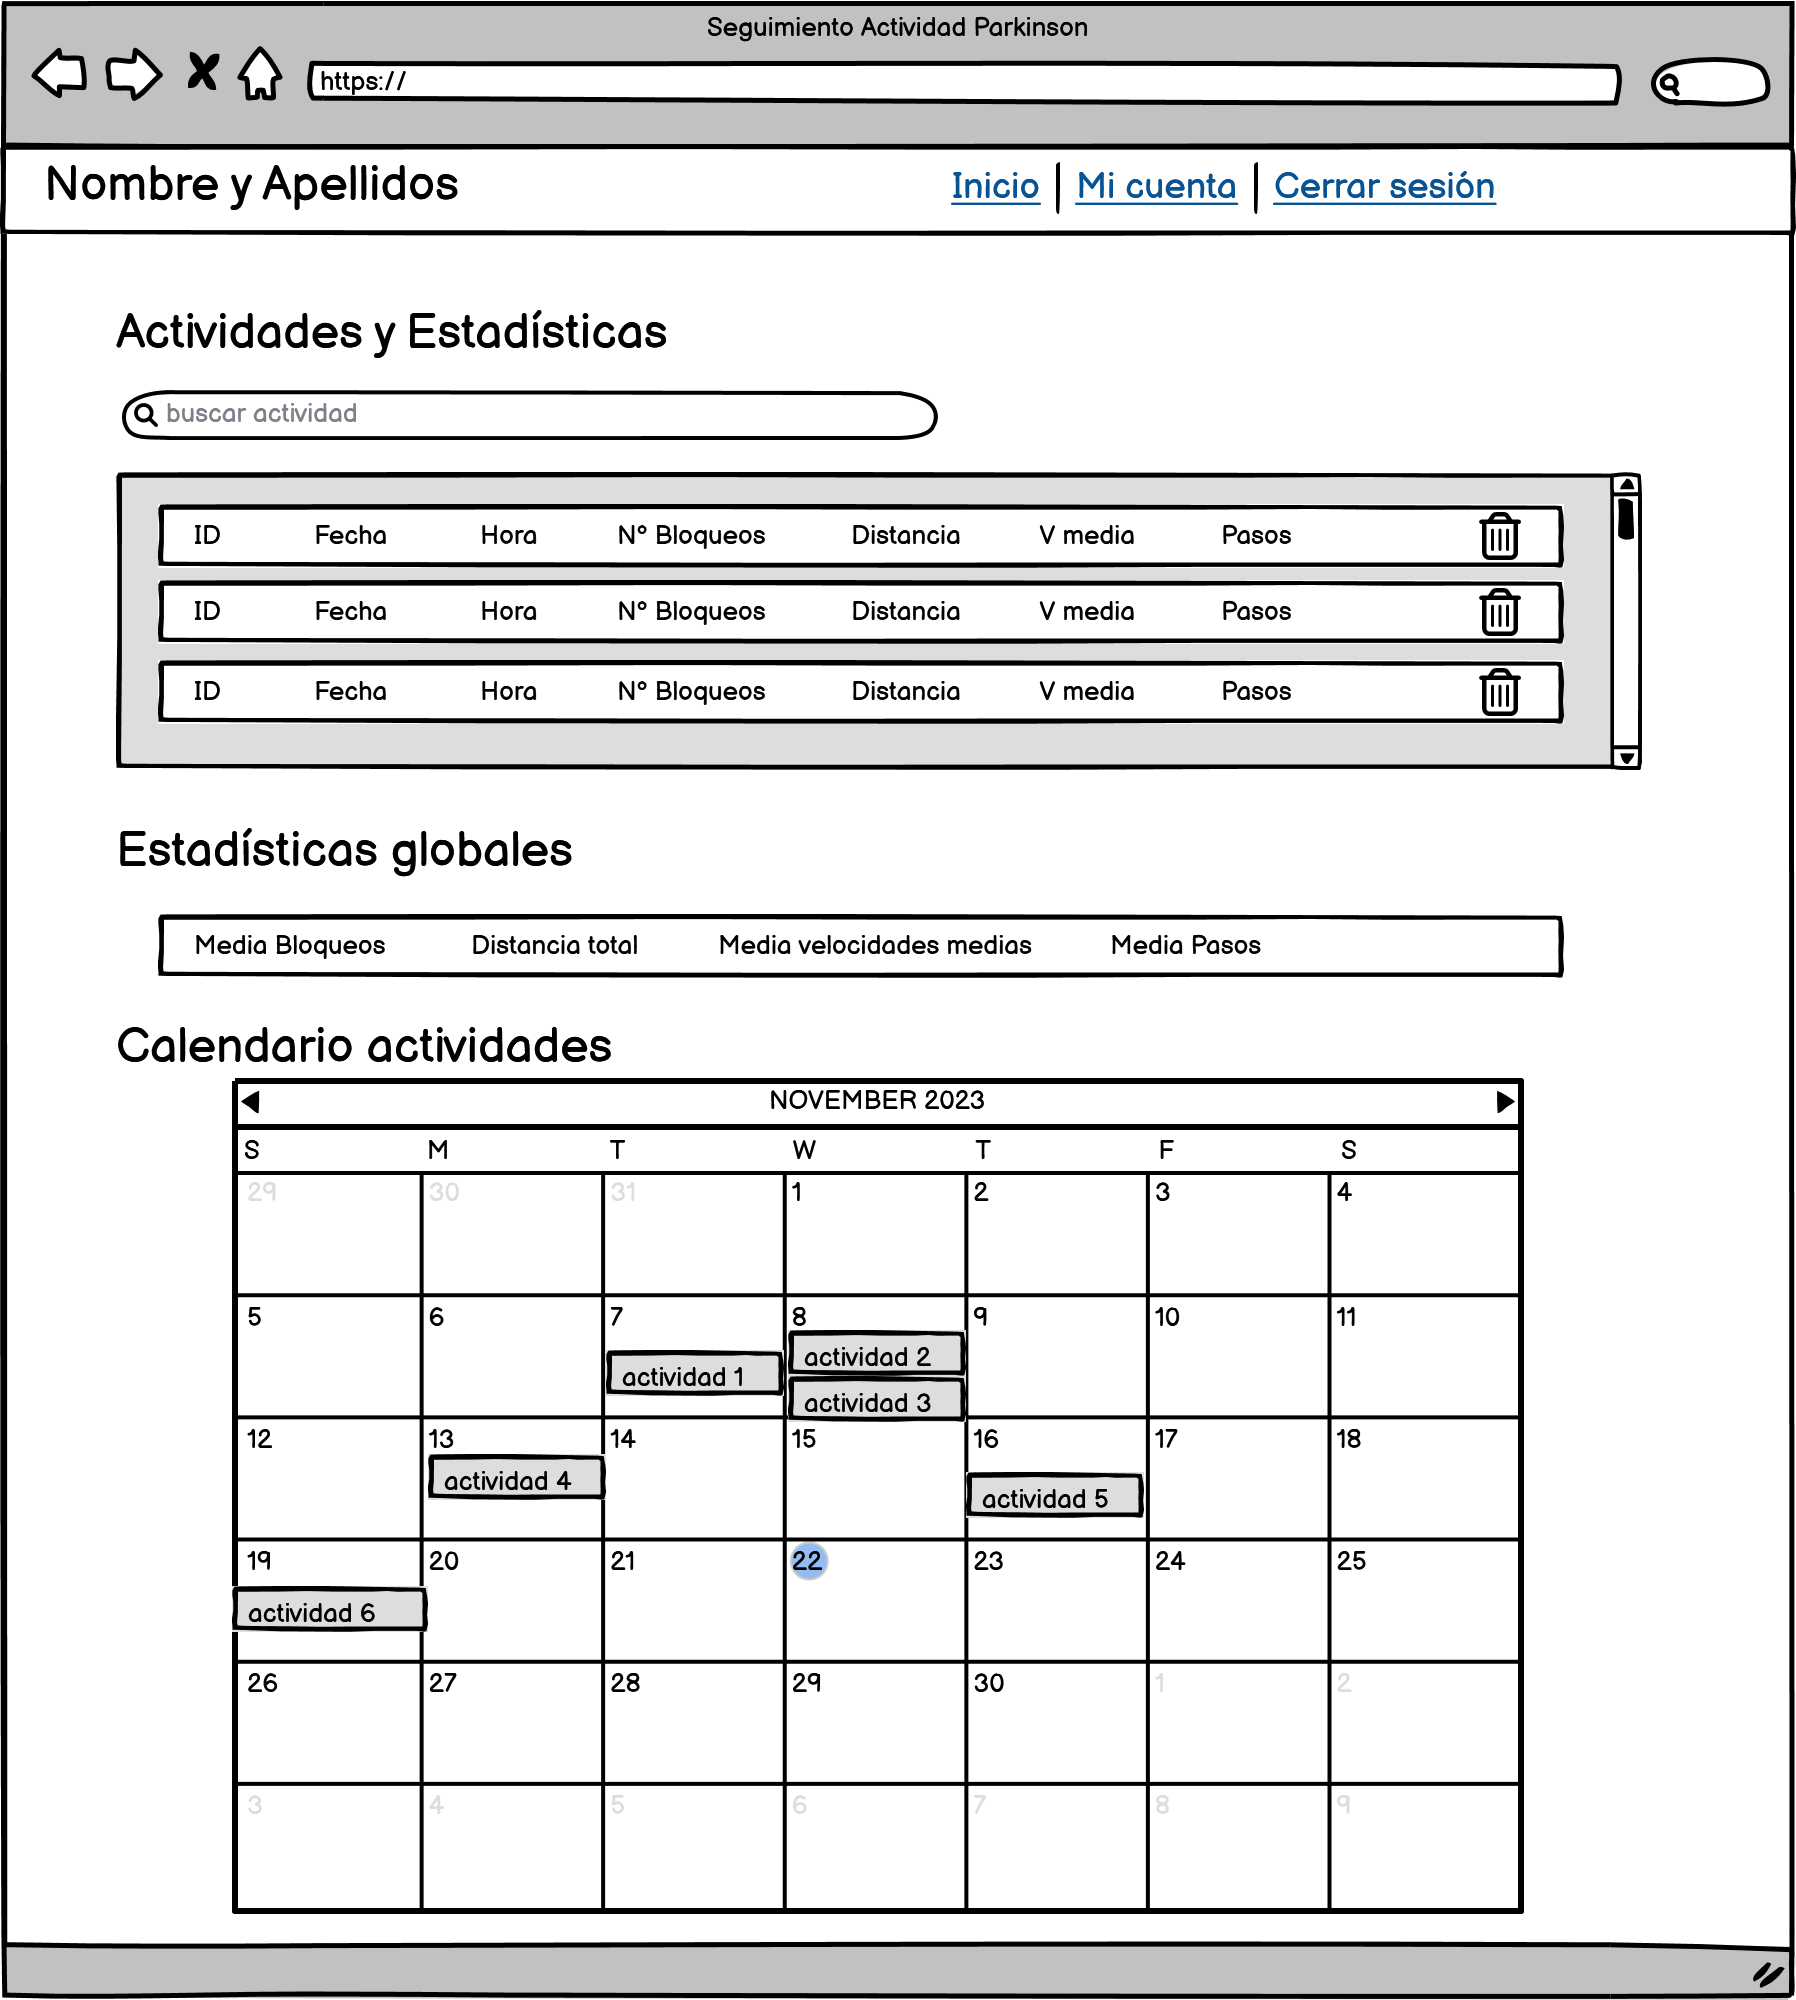
\includegraphics[width=1\textwidth]{img/UI_Wireframes/UI_CU-23_Pac-Consultar actividades y estadísticas (Alternate 323x) (Alternate 323x).png}
    \caption{Consultar actividades y estadísticas (Paciente)}
    \label{fig:Consultar actividades y estadísticas (Paciente)}
\end{figure}

% Consultar actividades y estadísticas (Profesional)
\begin{figure}[h]
    \centering
    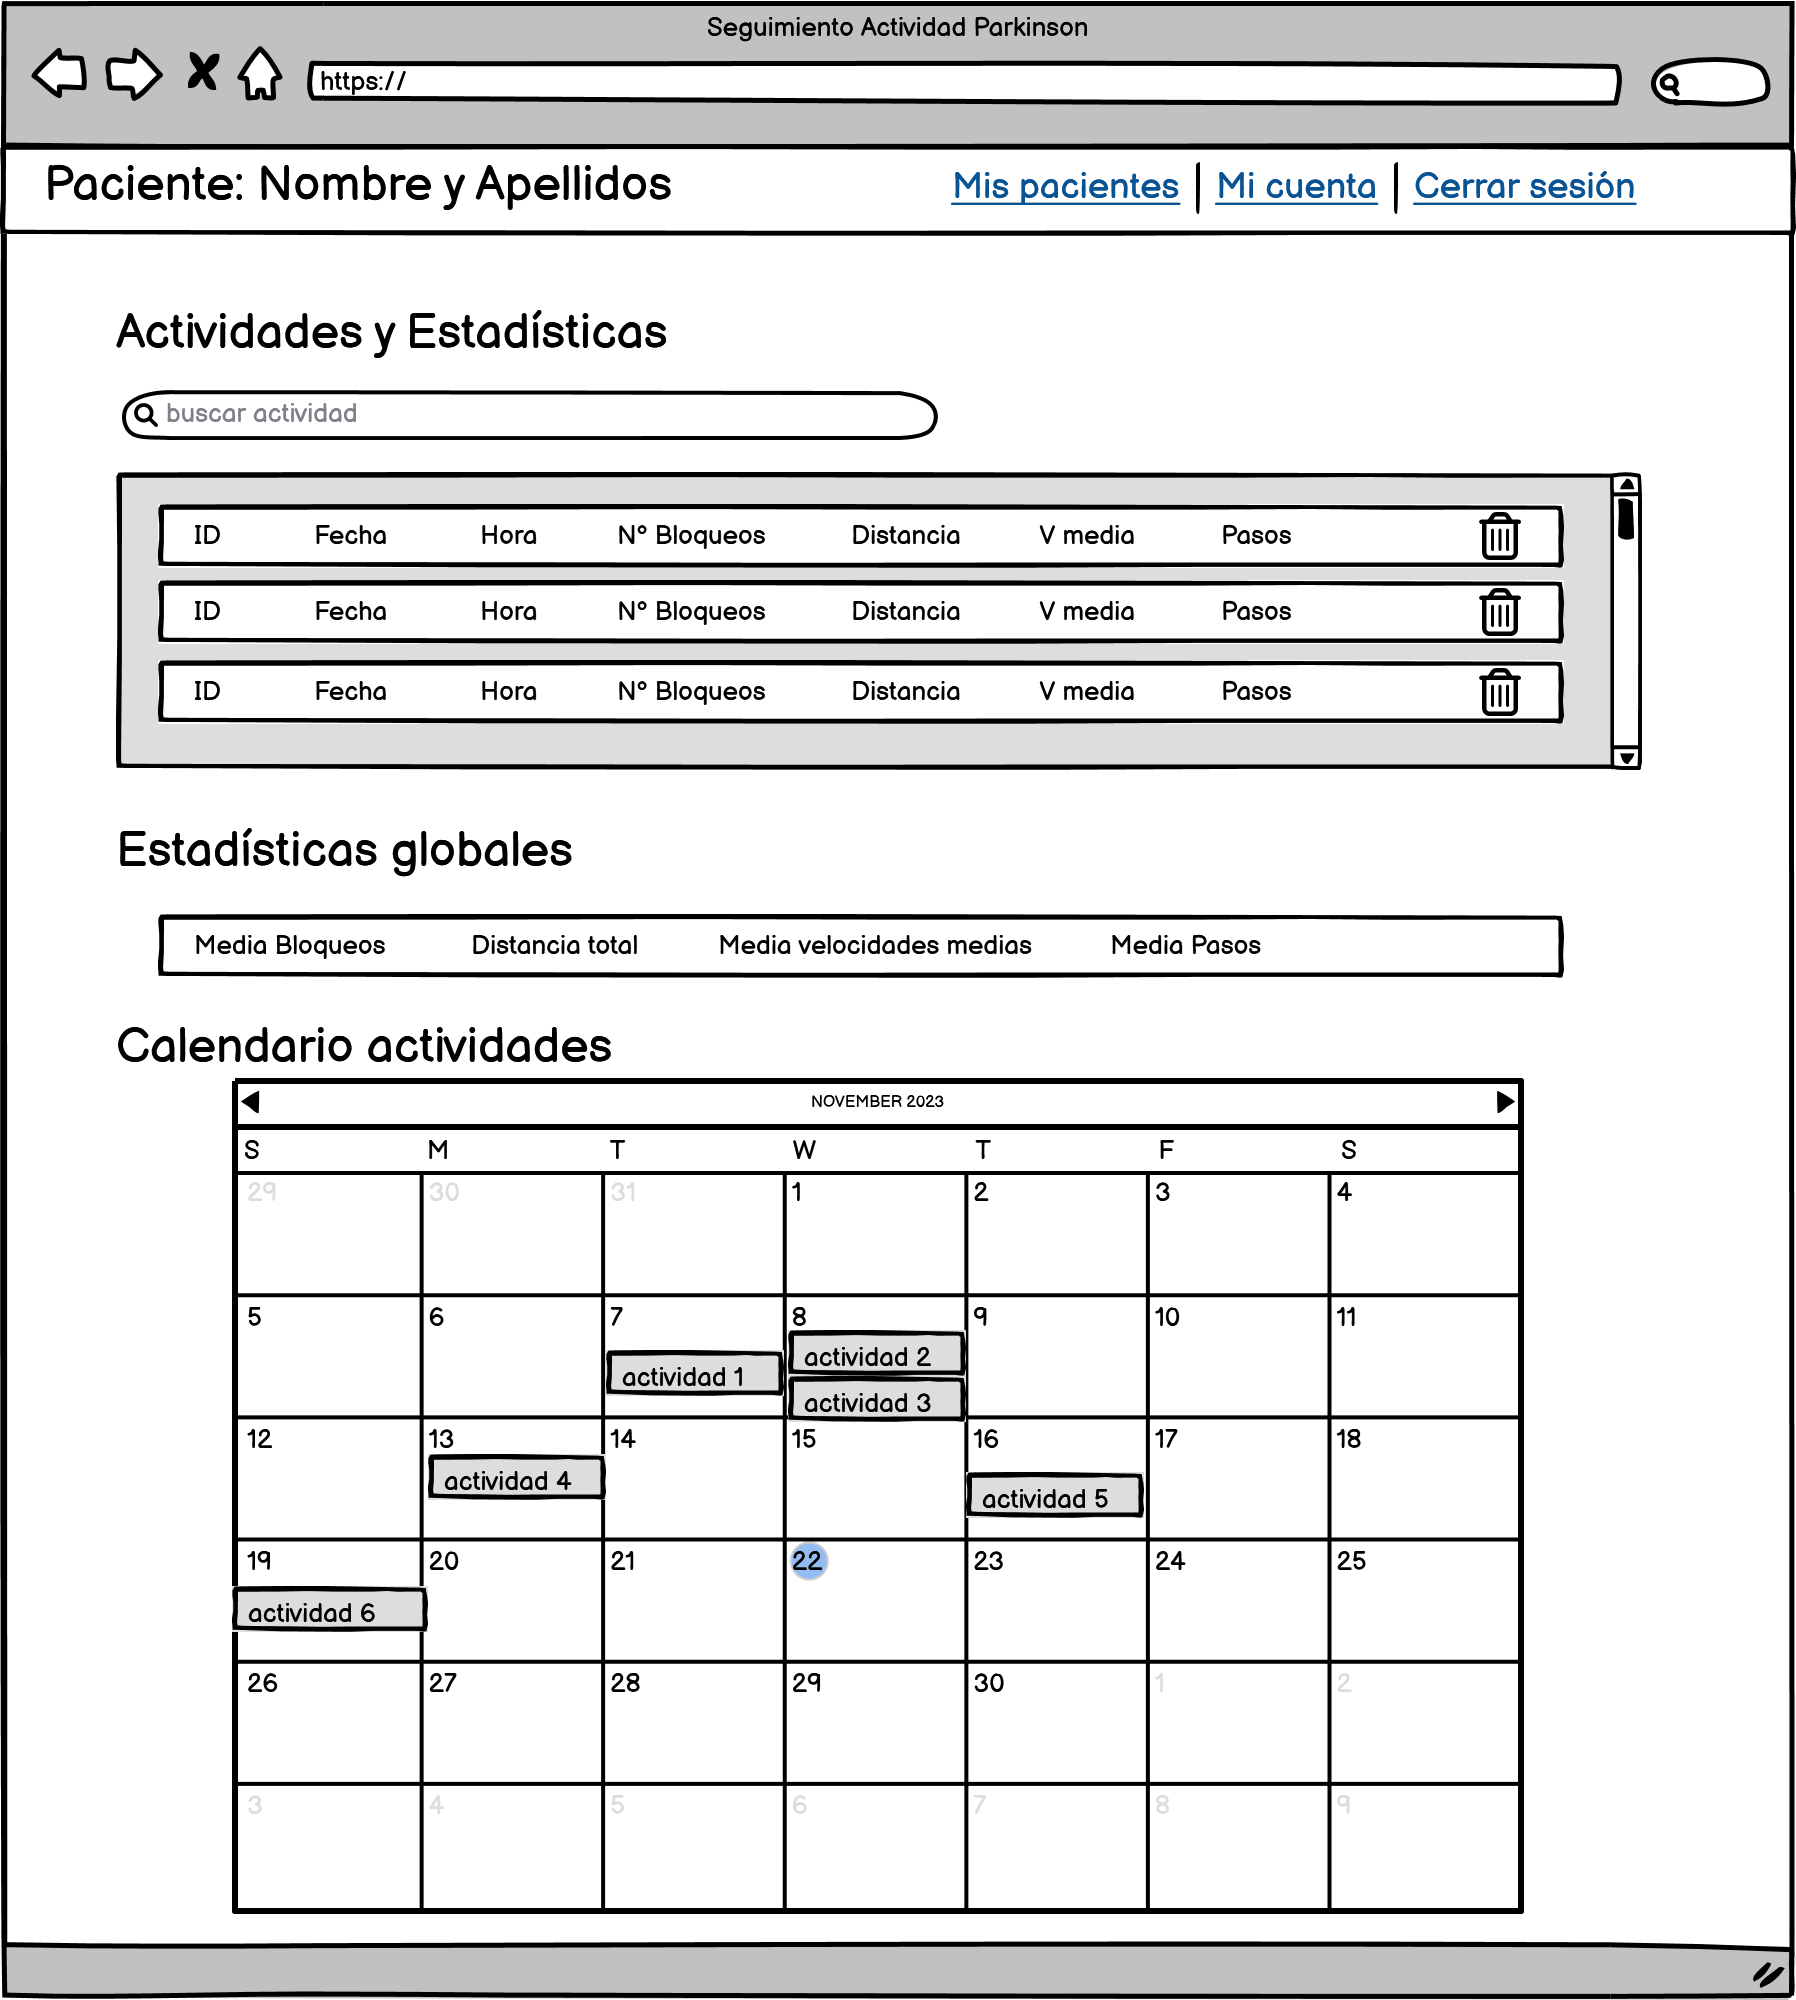
\includegraphics[width=1\textwidth]{img/UI_Wireframes/UI_CU-23_Prof-Consultar actividades y estadísticas.png}
    \caption{Consultar actividades y estadísticas (Profesional)}
    \label{fig:Consultar actividades y estadísticas (Profesional)}
\end{figure}

% Consulta y gestión de pacientes
\begin{figure}[h]
    \centering
    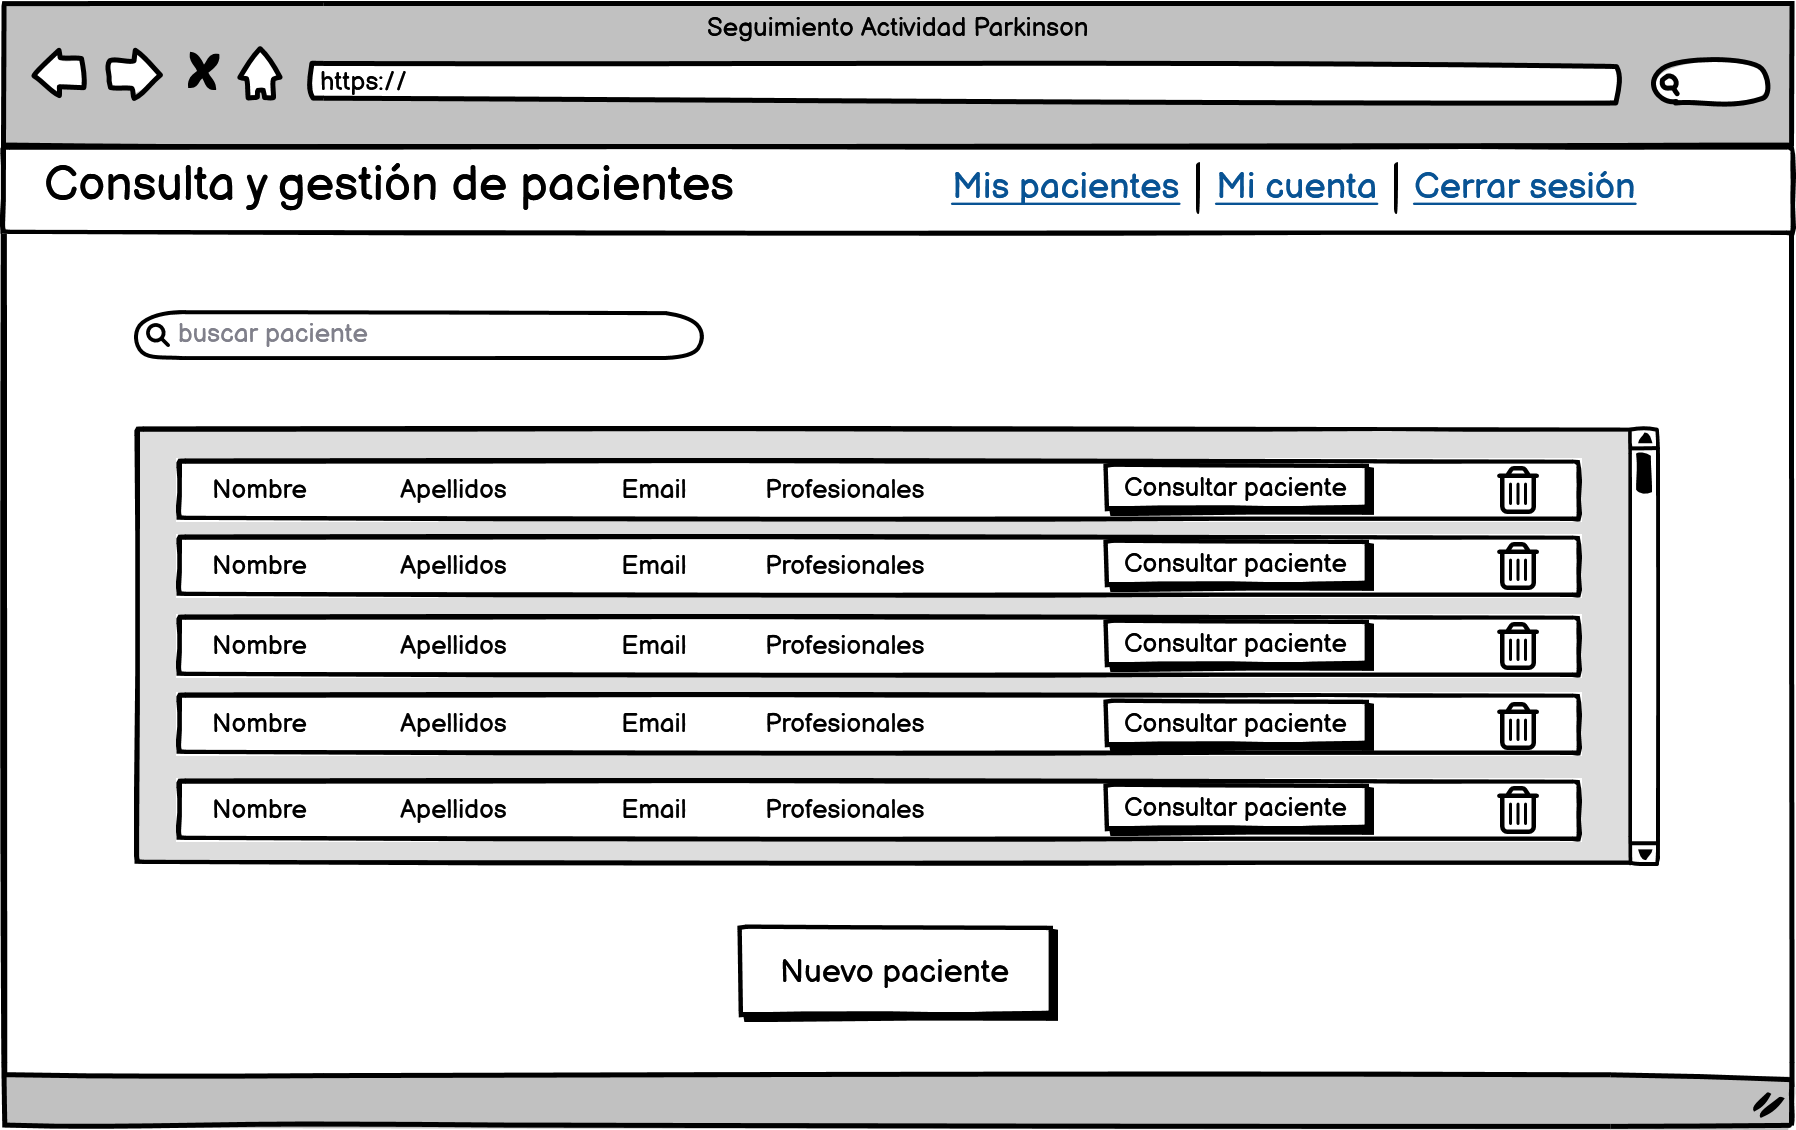
\includegraphics[width=1\textwidth]{img/UI_Wireframes/UI_CU-26_Consulta y gestion de pacientes.png}
    \caption{Consulta y gestión de pacientes}
    \label{fig:Consulta y gestión de pacientes}
\end{figure}

% Crear paciente
\begin{figure}[h]
    \centering
    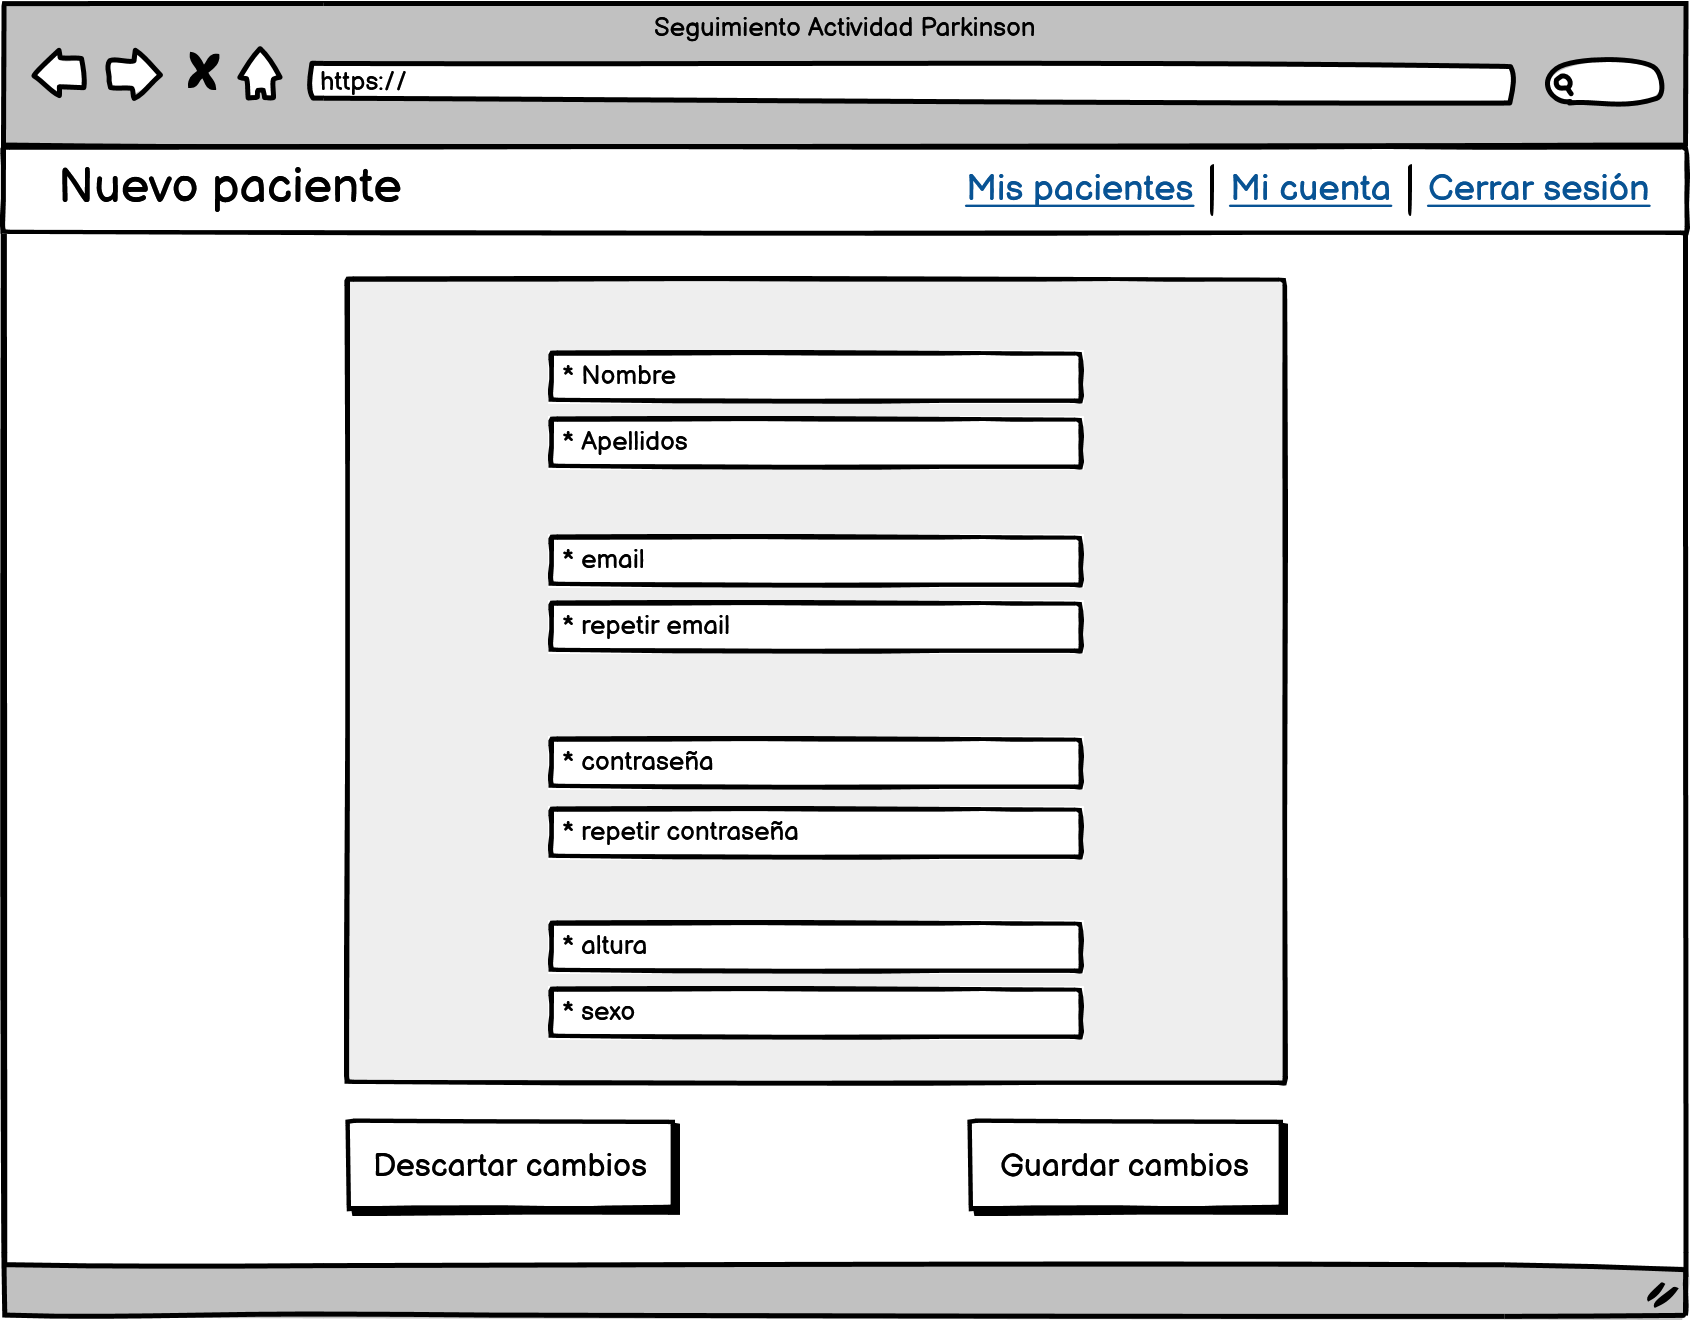
\includegraphics[width=1\textwidth]{img/UI_Wireframes/UI_CU-28_Crear paciente.png}
    \caption{Crear paciente}
    \label{fig:Crear paciente}
\end{figure}

% Visualizar paciente
\begin{figure}[h]
    \centering
    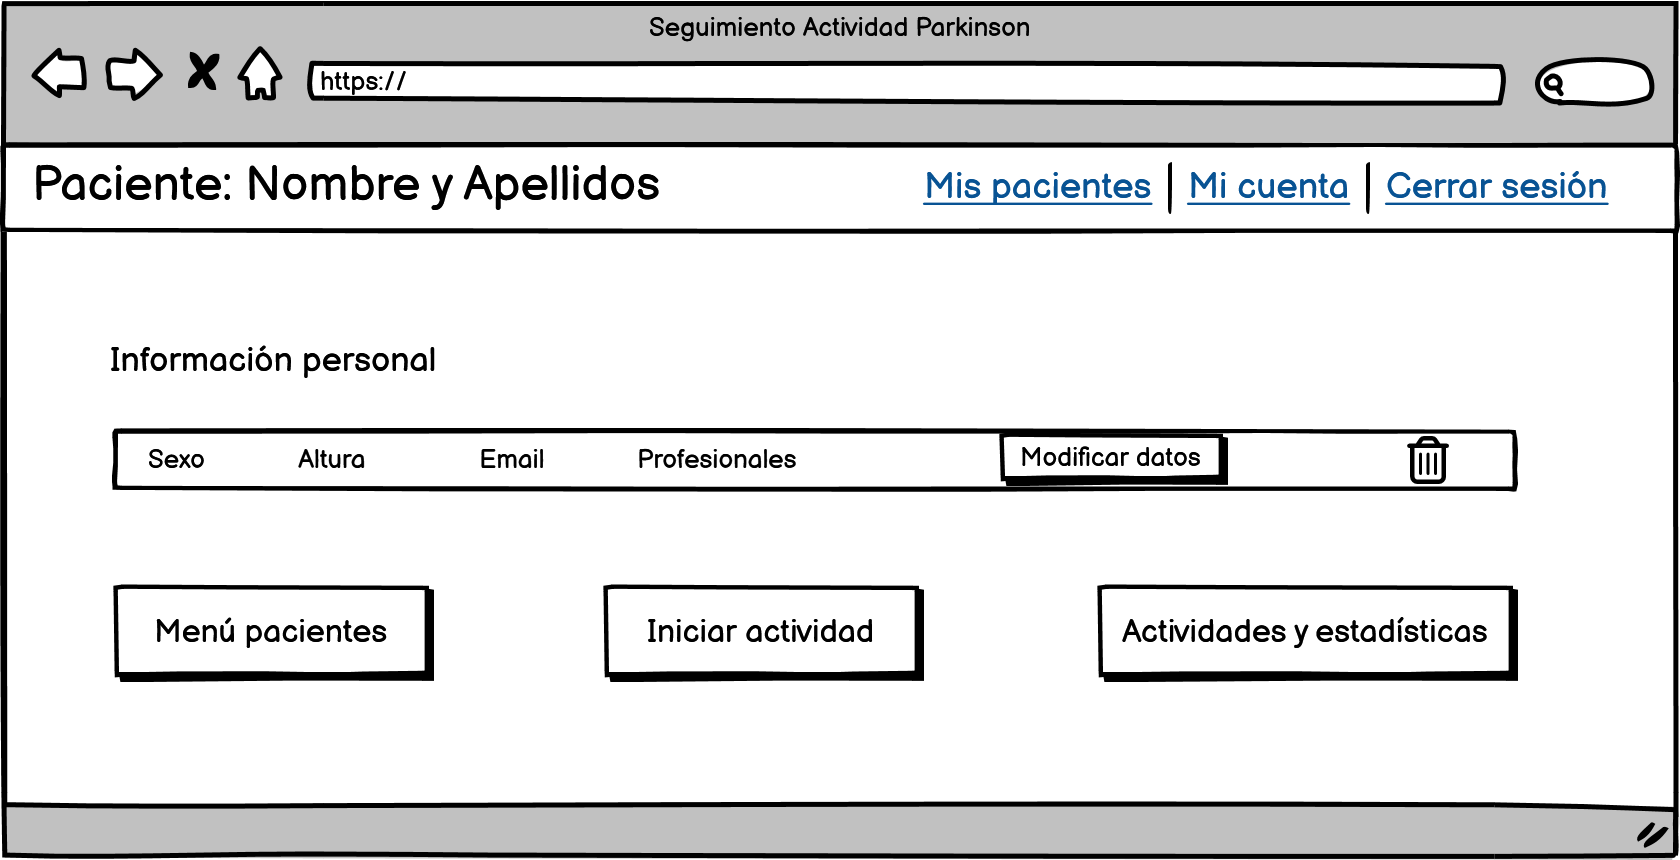
\includegraphics[width=1\textwidth]{img/UI_Wireframes/UI_CU-30_Visualizar paciente.png}
    \caption{Visualizar paciente}
    \label{fig:Visualizar paciente}
\end{figure}